\documentclass[uplatex,a4j,11pt,dvipdfmx]{jsarticle}
\usepackage{listings,jvlisting}
\bibliographystyle{junsrt}

\usepackage{url}

\usepackage{graphicx}
\usepackage{gnuplot-lua-tikz}
\usepackage{pgfplots}
\usepackage{tikz}
\usepackage{amsmath,amsfonts,amssymb}
\usepackage{bm}
\usepackage{siunitx}

\makeatletter
\def\fgcaption{\def\@captype{figure}\caption}
\makeatother
\newcommand{\setsections}[3]{
\setcounter{section}{#1}
\setcounter{subsection}{#2}
\setcounter{subsubsection}{#3}
}
\newcommand{\mfig}[3][width=15cm]{
\begin{center}
\includegraphics[#1]{#2}
\fgcaption{#3 \label{fig:#2}}
\end{center}
}
\newcommand{\gnu}[2]{
\begin{figure}[hptb]
\begin{center}
\input{#2}
\caption{#1}
\label{fig:#2}
\end{center}
\end{figure}
}

\begin{document}
\title{レーザー物理学 レポート No.8}
\author{82311971 佐々木良輔}
\date{}
\maketitle
\section*{問19}
図1において,媒質入射直前の電場を$E_1$, 出射直後の電場を$E_2$とすると
\begin{align}
  E_2=E_1e^{-\kappa kK+i\eta kL}=:\sqrt{G}E_1e^{i\eta kL}
\end{align}
これがリングを一周したとき$E_1$は
\begin{align}
  E_1=\sqrt{R}E_2e^{ik\Lambda}
\end{align}
(1)と(2)から
\begin{align}
  E_1=\sqrt{R}\sqrt{G}E_1e^{ik(\eta L+\Lambda)}
\end{align}
である.定常状態においては,この係数の絶対値が$1$になるべきなので
\begin{align}
  \begin{split}
    1&=\sqrt{R}\sqrt{G}\\
    &=\sqrt{R}\exp\left(\frac{\omega L|\mu_{12}|^2(N_2-N_1)}{2\varepsilon_0\hbar c}\frac{\gamma_2}{\delta^2+\gamma_2^2+\frac{\gamma_2}{\gamma_1}\Omega_0^2}\right)
  \end{split}
\end{align}
両辺の対数を取ると
\begin{align}
  \begin{array}{cc}
    &0=\cfrac{1}{2}\log R+\cfrac{\omega L|\mu_{12}|^2(N_2-N_1)}{2\varepsilon_0\hbar c}\cfrac{\gamma_2}{\delta^2+\gamma_2^2+\frac{\gamma_2}{\gamma_1}\Omega_0^2}\\
    \iff&\Omega_0^2=\left(\cfrac{\mu_{12} E}{\hbar}\right)^2=-\cfrac{\omega L|\mu_{12}|^2(N_2-N_1)}{\log R\varepsilon_0\hbar c}\gamma_1-\cfrac{\hbar^2}{\mu^2}\left(\cfrac{\gamma_1}{\gamma_2}\delta^2-\gamma_1\gamma_2\right)\\
    \iff&I=\cfrac{\varepsilon_0cE^2}{2}=-\cfrac{\omega L(N_2-N_1)\hbar\gamma_1}{\log R\varepsilon_0c}-\cfrac{\varepsilon_0c\hbar^2}{2|\mu_{12}|^2}\left(\cfrac{\gamma_1}{\gamma_2}\delta^2-\gamma_1\gamma_2\right)
  \end{array}
\end{align}
したがって$I=0$, $\delta=0$のときの反転分布数,すなわち閾値は
\begin{align}
  N_2-N_1=-\log R\frac{c\varepsilon_0\hbar\gamma_2}{|\mu_{12}|^2\omega L}
\end{align}
となる.またこのレーザーの発振周波数は(3)式の位相部分が$2\pi$の整数倍であれば良いので
\begin{align}
  k(\eta L+\Lambda)=2n\pi
\end{align}
ここで(5)より
\begin{align}
  \frac{|\mu_{12}|^2(N_2-N_1)}{2\varepsilon_0\hbar}\frac{\delta}{\delta^2+\gamma_2^2+\frac{\gamma_2}{\gamma_1}\Omega_0^2}=-\frac{1}{2}\log R\frac{c\delta}{\omega L\gamma_2}
\end{align}
なので
\begin{align}
  \begin{split}
    \eta&=1+\frac{|\mu_{12}|^2(N_2-N_1)}{2\varepsilon_0\hbar}\frac{\delta}{\delta^2+\gamma_2^2+\frac{\gamma_2}{\gamma_1}\Omega_0^2}\\
    &=1-\frac{c\delta}{2\omega L\gamma_2}\log R
  \end{split}
\end{align}
したがって(7)は$k=\omega/c$, $\delta=\omega-\omega_0$を用いると
\begin{align}
  \frac{\omega L}{c}\left(1-\frac{c\delta}{2\omega L\gamma_2}\log R\right)+\frac{\omega\Lambda}{c}=2n\pi\\    
\end{align}
更に$\omega_c=n\pi c/(L+\Lambda)$を用いると
\begin{align}
  \begin{array}{cc}
    &\omega L-\cfrac{c(\omega-\omega_0)}{2\gamma_2}\log R+\omega\Lambda=2\omega_c(L+\Lambda)\\
    \iff&\omega\left(L+\Lambda-\cfrac{c}{2\gamma_2}\log R\right)=2\omega_c(L+\Lambda)-\cfrac{c\omega_0}{2\gamma_2}\log R\\
    \iff&\omega=\cfrac{2\omega_c(L+\Lambda)-\frac{c\omega_0}{2\gamma_2}\log R}{L+\Lambda-\frac{c}{2\gamma_2}\log R}
  \end{array}
\end{align}
と求まる.
\begin{center}
  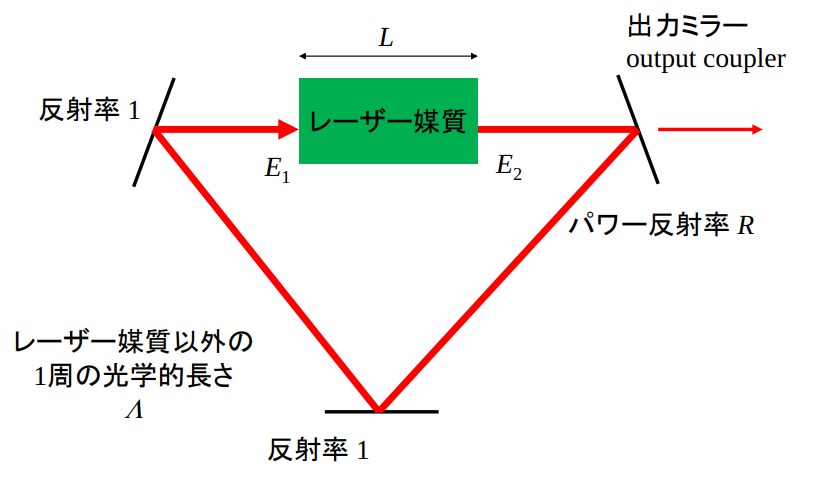
\includegraphics[width=10cm]{ring.png}
  \fgcaption{リング型共振器(授業スライドより引用)}
\end{center}
\end{document}